\usetikzlibrary{arrows.meta,calc}
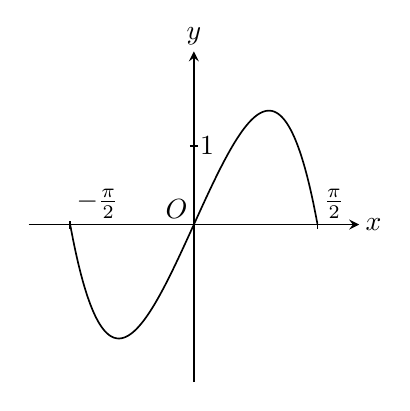
\begin{tikzpicture}[x=1cm,y=1cm,line width=.6pt,>=stealth]
\draw[->] (-2.1,0)--(2.1,0) node[right,inner sep=0pt,xshift=2pt] {$x$};
\draw[->] (0,-2.0)--(0,2.2) node[above,inner sep=0pt,yshift=2pt] {$y$};
\draw (-1.5708,-0.05)--(-1.5708,0.05);
\node[above right,inner sep=0pt,xshift=2pt,yshift=2pt] at (-1.5708,0) {$-\frac{\pi}{2}$};
\draw (1.5708,-0.05)--(1.5708,0.05);
\node[above right,inner sep=0pt,xshift=2pt,yshift=2pt] at (1.5708,0) {$\frac{\pi}{2}$};
\draw (-0.05,1)--(0.05,1);
\node[right,inner sep=0pt,xshift=2pt] at (0,1) {$1$};
\node[above left,inner sep=0pt,xshift=-2pt,yshift=2pt] at (0,0) {$O$};
\draw[domain=-1.5708:1.5708,samples=160] plot (\x,{(3^\x-3^(-\x))*cos(deg(\x))});
\end{tikzpicture}
